%%=============================================================================
%% Methodologie
%%=============================================================================

\chapter{\IfLanguageName{dutch}{Methodologie}{Methodology}}%
\label{ch:methodologie}

%% TODO: In dit hoofstuk geef je een korte toelichting over hoe je te werk bent
%% gegaan. Verdeel je onderzoek in grote fasen, en licht in elke fase toe wat
%% de doelstelling was, welke deliverables daar uit gekomen zijn, en welke
%% onderzoeksmethoden je daarbij toegepast hebt. Verantwoord waarom je
%% op deze manier te werk gegaan bent.
%% 
%% Voorbeelden van zulke fasen zijn: literatuurstudie, opstellen van een
%% requirements-analyse, opstellen long-list (bij vergelijkende studie),
%% selectie van geschikte tools (bij vergelijkende studie, "short-list"),
%% opzetten testopstelling/PoC, uitvoeren testen en verzamelen
%% van resultaten, analyse van resultaten, ...
%%
%% !!!!! LET OP !!!!!
%%
%% Het is uitdrukkelijk NIET de bedoeling dat je het grootste deel van de corpus
%% van je bachelorproef in dit hoofstuk verwerkt! Dit hoofdstuk is eerder een
%% kort overzicht van je plan van aanpak.
%%
%% Maak voor elke fase (behalve het literatuuronderzoek) een NIEUW HOOFDSTUK aan
%% en geef het een gepaste titel.

In de initiële fase van dit onderzoek, de literatuurstudie, wordt de focus gelegd op het verzamelen van bestaande kennis 
en onderzoek op het gebied van webapplicatiebeveiliging, pentesting-tools en frameworks, met een specifieke nadruk op 
WordPress en Laravel. Deze fase is van cruciaal 
belang om een stevige basis te leggen voor mijn onderzoek en om de context en achtergrond van het onderwerp volledig te 
begrijpen.

Om dit te bereiken, worden verschillende bronnen geraadpleegd, waaronder wetenschappelijke artikelen, boeken  
en rapporten van bekende instellingen en experts op het gebied van cybersecurity. 
Ook worden zoekopdrachten uitgevoerd in diverse academische databases, zoals PubMed, research gate en 
Google Scholar om relevante en onderbouwde literatuur op te nemen in de studie. Deze literatuur is grondig geanalyseerd en 
samengevat, waarbij de nadruk werd gelegd op recente ontwikkelingen, trends en mogelijke tekortkomingen in de bestaande markt.
Ook wordt in dit deel het globale aspect van cybersecutiy onder de loep genomen waardoor er een zeer duidelijk begrip 
is van de noden en hoe hierop een antwoord wordt gegeven.

\section{\IfLanguageName{dutch}{Requirements Analyse}{Requirements analysis}}
De requirements analyse vormt een cruciaal luik en beschrijft de methoden en technieken die worden toegepast 
voor het uitvoeren van penetratietests. In deze studie worden deze toegepast op twee 
verschillende webomgevingen met name een WordPress CMS-framework en een Laravel-applicatie. Het doel van deze tests is om kwetsbaarheden te identificeren, te 
analyseren en de effectiviteit van de beveiligingsmaatregelen en aanvalstrategieën in de verschillende omgevingen te vergelijken.
Deze twee webomgevingen zijn geselecteerd op basis van hun populariteit en relevantie voor kleine tot middelgrote bedrijven 
zoals webdevelopment firma Sinergio, die de partner en co-promotor is in dit onderzoek.

Voor de start van deze studie worden eerst de nodige keuzes en methodieken verklaard en verantwoord. De manier waarop deze keuzes zijn gemaakt, wordt eveneens 
besproken, zodat dit in een latere fase van het onderzoek kan worden uitgevoerd.

Dit onderzoek is opgesplitst in twee delen waarbij in de initiële fase gefocust wordt op de keuze van de meest passende pentesting tool 
aan de hand van vooropgestelde criteria. Hierop gebaseerd worden drie pentestingtools gekozen die op hun beurt worden vergeleken met elkaar 
zodat er in de tweede fase van het onderzoek op een solide basis kan worden verder gebouwd. In deze fase zal met de geselecteerde 
tool dertien pentests worden afgenomen op de omgevingen waarbij er binnen de testen op een wordpress CMS systeem nog onderscheid zal worden gemaakt 
tussen een versie met en een versie zonder beveiligingsplugin.

\subsection{\IfLanguageName{dutch}{Keuze van pentesttools}{choice of pentesttools}}
Voor dit onderzoek is het van 
belang dat tools worden gebruikt met vergelijkbare functionaliteiten, maar met verschillende intrinsieke accenten om te bepalen welke 
tool het meest geschikt is binnen de hiervoor besproken scenarios. In het kader van deze proef is het belangrijk dat er voldoende onderscheid is tussen de tools 
die worden vergeleken, zodat in de conclusie duidelijk wordt welke pentesttool het meest geschikt en toepasselijk is in deze context. 
Pentesting-tools zoals Nmap of Wireshark zijn vooral gericht op het testen van netwerken en  zijn daarom minder van toepassing. Er wordt
gediversifieerd in de selectie van de beschikbare tools door te selecteren in de open source omgeving en minstens één die niet open-source is, waarbij de gratis versie wordt 
verkozen. Aangezien de pentesttool kost efficiënt dient te zijn is het de voornaamste optie een open-source tool te gebruiken, daarom 
is dit een factor waarop vergeleken wordt door de vergelijking op te stellen tussen een gratis versie van een pentesting tool en een open-source tool. 
Tevens wordt één tool geselecteerd waarbij de pentesting-capaciteiten verder gaan dan alleen het testen van webapplicaties, met een 
uitgebreider scala aan mogelijkheden zoals het testen van netwerken of mobiele applicaties. Zodat duidelijk wordt dat dit de
de doeltreffendheid van de pentesten bevordert.

Op basis van deze criteria worden onderstaande pentest toepassingen weerhouden:
\begin{itemize}
    \item Metasploit: open-source software met en een uitgebreider scala aan functionaliteiten die niet enkel voor web applicatie testing dienen.
    \item Burp suite: geen open-source software die is alleen dient voor het testen van web applicaties.
    \item OWASP ZAP: open-source software die alleen gebruikt wordt voor het testen van web applicaties.
\end{itemize}


De daaropvolgende keuze tussen de drie weerhouden pentesttools is gebaseerd op vooraf vastgestelde globale criteria, waarbij de nadruk ligt op welke tool het meest 
geschikt is voor het testen van de opgezette omgevingen (wordpress CMS en Laravel applicatie). Deze criteria omvatten:
\begin{itemize}
    \item De omvang van het scala aan capaciteiten en functionaliteiten voor het testen van webapplicaties.
    \item Resourcegebruik met name CPU-, geheugen- en netwerkgebruik.
    \item Ondersteuning door de community, door de gemiddelde antwoordtijd van reacties van 20 laatste openstaande issues te vergelijken.
\end{itemize}

Bij de selectie van de te weerhouden pentesting-tool voor dit onderzoek wordt eerst een eigen analyse gemaakt op basis van deze bovenstaande criteria. 
Nadien wordt een analyse gemaakt van gebruikerservaringen van derden. Dit gebeurt aan de hand van beoordelingen en recenties van 
verschillende gebruikers, waarbij de pro's en contra's die de reviewers vermelden in overweging word genomen. De vergelijking 
van derden is belangerijk, aangezien het niet haalbaar is om een volledig framework 
autonoom te evalueren zonder rekening te houden met de mening van anderen. Daarom is het van groot belang om ook de conclusies van externe partijen mee te nemen, die mogelijk andere 
aspecten hebben waargenomen. Op basis van 
deze laatste analyse zal worden geconcludeerd welke pentesting-tool het meest geschikt is voor gebruik in deze context.

\subsection{\IfLanguageName{dutch}{Aanpak van web omgevingen}{Use of web enviroments}}
Voorafgaand aan de uitvoering van de penetratietests worden in samenspraak met de partner van deze bachelorproef, Sinergio, drie 
webapplicaties opgezet waarop de tests later worden uitgevoerd. Om de business impact minimaal te houden wordt hiertoe een 
aparte test-server opgezet. Alle tests worden overigens uitgevoerd in overeenstemming met de ethische 
richtlijnen voor cybersecurityonderzoek, waarbij de integriteit van de geteste systemen vooropstaat. De te testen 
webapplicaties zijn de onderstaande en bereikbaar via de link:

\begin{itemize}
    \item Wordpress applicatie met beveiligingsplugins: \url{http://testlevi.abako.be/}
    \item Wordpress applicatie zonder beveiligingsplugins: \url{http://testlevi.abako.be/}
    \item Laravel applicatie: \url{https://solfo.abako.be/}
\end{itemize}

Binnen het onderzoek wordt voornamelijk gekeken naar welke omgeving het meest robuust is tegen verschillende pentestaanvallen. 
Het is daarom belangrijk om de juiste kwetsbaarheden te testen, zodat er een correcte en volledige conclusie kan worden 
getrokken. De geselecteerde kwetsbaarheden zijn gebaseerd op de OWASP Top 10, een lijst van de tien belangrijkste 
kwetsbaarheden binnen de cybersecuritywereld. Niet alle kwetsbaarheden uit deze lijst kunnen echter worden getest met de 
gekozen pentesting-tool. Om deze reden is ervoor gekozen om ook onderzoek uit te voeren naar externe aanvallen die momenteel veel 
aandacht krijgen. Dit heeft geleid tot de volgende uitgevoerde pentests:

\begin{itemize}
    \item SQL injection aanval
    \item Brute force aanval
    \item Broken authentication
    \item Sensitive data exposure
    \item Broken access control
    \item Security misconfiguration
    \item Cross site scripting
    \item Insecure deserialization
    \item Using components with known vulnerabilities
    \item Insufficient logging \& monitoring 
    \item client side logica
\end{itemize}

\begin{tabular}{ | c | c | c | c |}
    \hline			
    webapplicatie & gelukte pentests & mislukte pentests & percentage gelukt \\
    \hline  
    wordpress zonder plugin & & & \\
    wordpress met plugin & & & \\
    laravel &  &  & \\
    \hline
\end{tabular}

Alle resultaten van de tests worden verzameld en gedocumenteerd aan de hand van bovenstaande tabel. De data wordt geanalyseerd 
om de ernst en de impact van elke gevonden kwetsbaarheid te bepalen. Deze analyse helpt niet alleen bij 
het identificeren van de zwakke punten binnen elke webomgeving, maar ook bij het vergelijken van de 
veiligheid tussen de verschillende systemen.

\section{\IfLanguageName{dutch}{Keuze van Penetratietesttools}{Selection of pentesttools}}
In het kader van dit onderzoek naar de beveiliging van de drie verschillende webomgevingen is de keuze van 
de juiste penetratietesttools cruciaal. De geselecteerde tools zijn 
Metasploit, Burp Suite en OWASP ZAP, waarbij hierna wordt toegelicht wat hen bijzonder geschikt maken voor dit onderzoek.
\begin{figure}
    \centering
    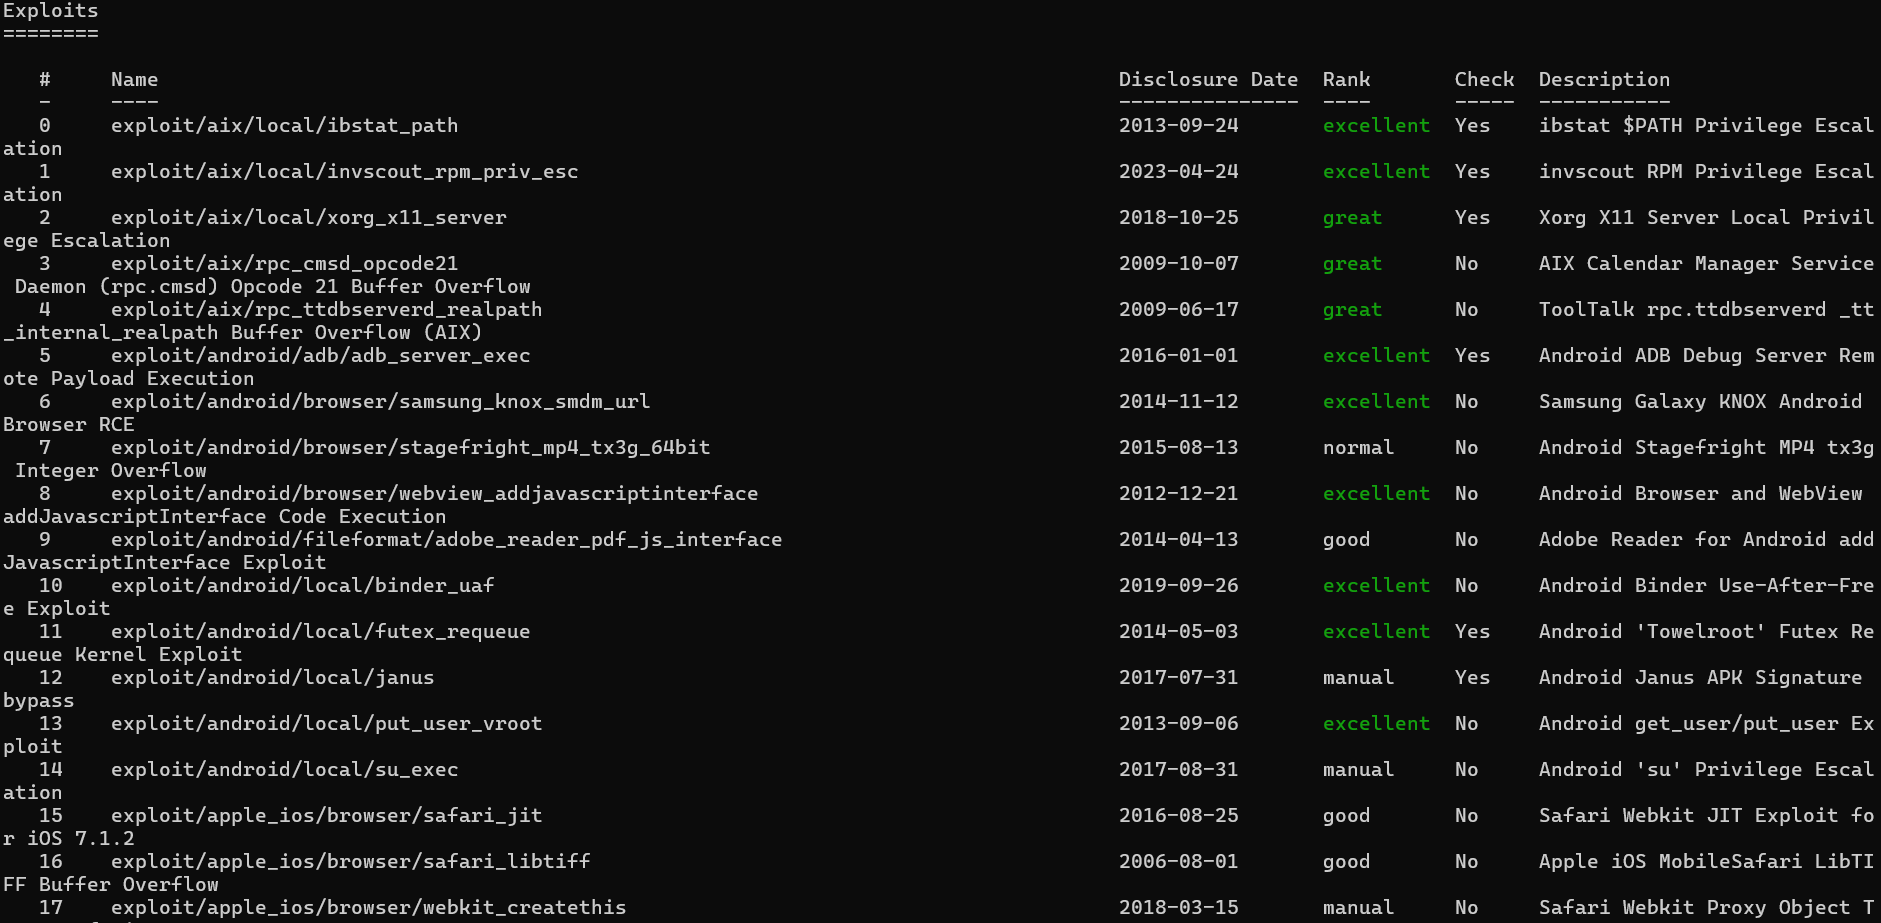
\includegraphics[height=0.3\textheight]{metasploit_exploit_db.png}
    \caption[exploitation database van metasploit]{exploitation database van metasploit}
    \label{fig:exploitatie_db}
\end{figure}
\subsection{\IfLanguageName{dutch}{Metasploit}{Metasploit}}
Metasploit is een van de meest uitgebreide security frameworks voor het uitvoeren van penetratietests en staat bekend om 
zijn robuuste exploit-database, waarvan een deel te zien is op de bovenstaande foto \ref{fig:exploitatie_db} en zoals vermeld is in het hoofdstuk \nameref{sec:Pentesting tools} van de 
literatuurstudie. Het framework biedt het vermogen om specifieke exploits te gebruiken die zijn afgestemd op gedetecteerde 
kwetsbaarheden. Metasploit biedt bovendien geautomatiseerde exploitatie-technieken, die essentieel zijn voor het identificeren 
van beveiligingsrisico's in geavanceerde frameworks zoals Laravel. Daarnaast ondersteunt Metasploit de ontwikkeling van 
aangepaste exploits en biedt het integratie met andere tools zoals Nmap en Wireshark, wat de veelzijdigheid en het 
gebruiksgemak verder vergroot. Een andere belangrijke functie is de mogelijkheid om uitgebreide rapportages te genereren, 
wat cruciaal is voor het documenteren van bevindingen en het communiceren van resultaten naar Sinergio en stakeholders. Dankzij de grote 
community en voortdurende updates blijft Metasploit relevant en actueel, wat het tot een essentieel hulpmiddel maakt in het 
testen van web applicaties.

\subsection{\IfLanguageName{dutch}{Burp Suite}{Burp Suite}}
Burp Suite is een platform voor het testen van de beveiliging van webapplicaties en is bijzonder effectief voor 
het analyseren van HTTP-verkeer en het uitvoeren van geavanceerde webaanvallen. Zoals besproken in het hoofdstuk \nameref{sec:Pentesting tools} 
van de literatuurstudie, biedt Burp Suite uitgebreide functionaliteiten die essentieel zijn voor een grondige beveiligingsanalyse 
van webomgevingen. Dankzij zijn vermogen om verzoeken te onderscheppen, te manipuleren en opnieuw te versturen, kunnen 
testers nauwkeurig de robuustheid beoordelen van beveiligingsmaatregelen zoals firewalls en inbraakdetectiesystemen die via 
plugins worden geïmplementeerd. 

De Community Edition van Burp Suite biedt basisfunctionaliteiten, zoals de proxy en repeater, 
waarmee handmatige testactiviteiten kunnen worden uitgevoerd. Met de Proxy kunnen testers bijvoorbeeld HTTP(S)-verkeer 
onderscheppen en manipuleren voordat het de server bereikt, wat hen in staat stelt om kwetsbaarheden zoals injection flaws 
te ontdekken door bijvoorbeeld SQL-commando's in te voegen in velden die normaal gesproken niet kwetsbaar lijken. Testers 
kunnen ook cookies en headers inspecteren en aanpassen, wat helpt bij het ontdekken van session hijacking of cookie 
manipulation kwetsbaarheden.

De Repeater stelt testers in staat om specifieke HTTP-verzoeken meerdere keren handmatig te versturen, waarbij elke keer 
kleine wijzigingen kunnen worden aangebracht. Dit is bijzonder nuttig voor het testen van de robuustheid van 
input-validatiesystemen en het verfijnen van aanvallen zoals Cross-Site Scripting (XSS) of Brute force attack. Door 
herhaaldelijk verzoeken met variaties te versturen, kunnen testers de reacties van de server analyseren en mogelijke 
kwetsbaarheden identificeren.

Hoewel de Community Edition beperkingen heeft ten opzichte van de 
commerciële edities, is het nog steeds een krachtig hulpmiddel voor basisbeveiligingsanalyses en een waardevolle aanvulling 
voor beginnende testers. De scanner in de Enterprise Edition van Burp Suite kan automatisch een breed scala aan kwetsbaarheden 
identificeren, wat tijd bespaart tijdens de testfase en zorgt voor een grondige evaluatie van de beveiligingsstatus.

\subsection{\IfLanguageName{dutch}{OWASP ZAP}{OWASP ZAP}}
OWASP ZAP (Zed Attack Proxy) is een open-source tool die zich richt op het automatisch detecteren van beveiligingsfouten in 
webapplicaties tijdens het ontwikkelings- en testproces. Met ZAP's geïntegreerde scanner en intercepting proxy kunnen 
kwetsbaarheden zoals Cross-Site Scripting (XSS) en SQL-injectie eenvoudig worden opgespoord. ZAP biedt 
daarnaast dynamische analyse van applicaties in real-time, waardoor beveiligingsproblemen direct kunnen worden geïdentificeerd 
en aangepakt. De tool is bijzonder nuttig voor zowel ontwikkelaars als beveiligingsexperts, doordat het hen in staat stelt 
om continue beveiligingstesten uit te voeren tijdens de gehele levenscyclus van een webapplicatie. Dit zorgt ervoor dat 
OWASP ZAP een zeer aantrekkenlijke keuze is voor het ontwikkel team van Sinergio.
\begin{figure}
    \centering
    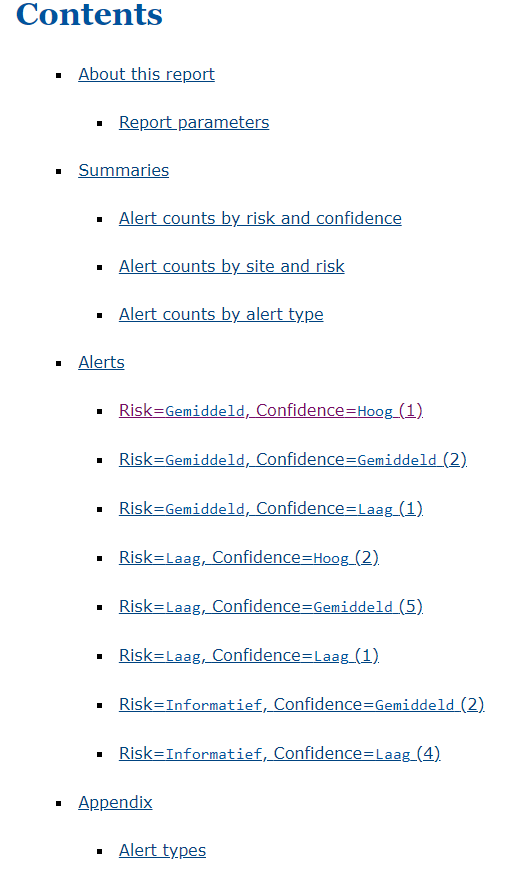
\includegraphics[height=0.3\textheight]{ZAP_report.png}
    \caption[voorbeeld rapportage van vanuit OWASP ZAP]{voorbeeld rapportage van vanuit OWASP ZAP}
    \label{fig:zap_report}
\end{figure}
ZAP is bovendien sterk uitbreidbaar dankzij zijn robuuste add-on marktplaats, waarmee gebruikers extra functionaliteiten 
kunnen toevoegen voor specifieke beveiligingstests. Een ander belangrijk aspect is de actieve en ondersteunende community 
rond OWASP ZAP, die regelmatig updates en nieuwe functies uitbrengt, waardoor de tool up-to-date blijft met de nieuwste 
beveiligingstrends en bedreigingen. ZAP biedt ook geautomatiseerde rapportagefuncties die gedetailleerde inzichten geven 
in de gevonden kwetsbaarheden zoals op bovenstaande foto \ref{fig:zap_report}. Dit is essentieel voor het documenteren van testresultaten en het verbeteren van de beveiliging 
van webapplicaties. 

\section{\IfLanguageName{dutch}{ Verkozen webomgevingen }{ chosen webenviroments }}
Voor de tests wordt gebruikgemaakt van het WordPress CMS-framework en Laravel. Deze frameworks zijn gekozen vanwege hun 
populariteit bij KMO's en middelgrote bedrijven zoals Sinergio. Binnen Sinergio wordt WordPress voornamelijk verkozen vanwege 
zijn grote populariteit, gebruiksvriendelijkheid en het feit dat het open-source is. Het brede scala aan plugins en de 
blijvende ondersteuning vanuit de community hebben Sinergio mede overtuigd om te kiezen voor WordPress. 
Laravel daarentegen is door Sinergio gekozen vanwege de eenvoud bij upgrades. Het is bijvoorbeeld mogelijk om websites 
te upgraden naar een nieuwere versie van Laravel zonder dat er gegevens verloren gaan. De kennis in verband met Laravel was 
reeds aanwezig binnen Sinergio waardoor de keuze voor dit framework snel gemaakt was. Ook de ingebouwde beveiligingsmaatregelen 
van Laravel, zoals de Eloquent ORM (hier word later op terug gekomen), hebben bijgedragen aan de keuze voor dit framework.

\subsection{\IfLanguageName{dutch}{Sinergio}{Sinergio}}
Sinergio is een KMO dat be

\begin{figure}
    \centering
    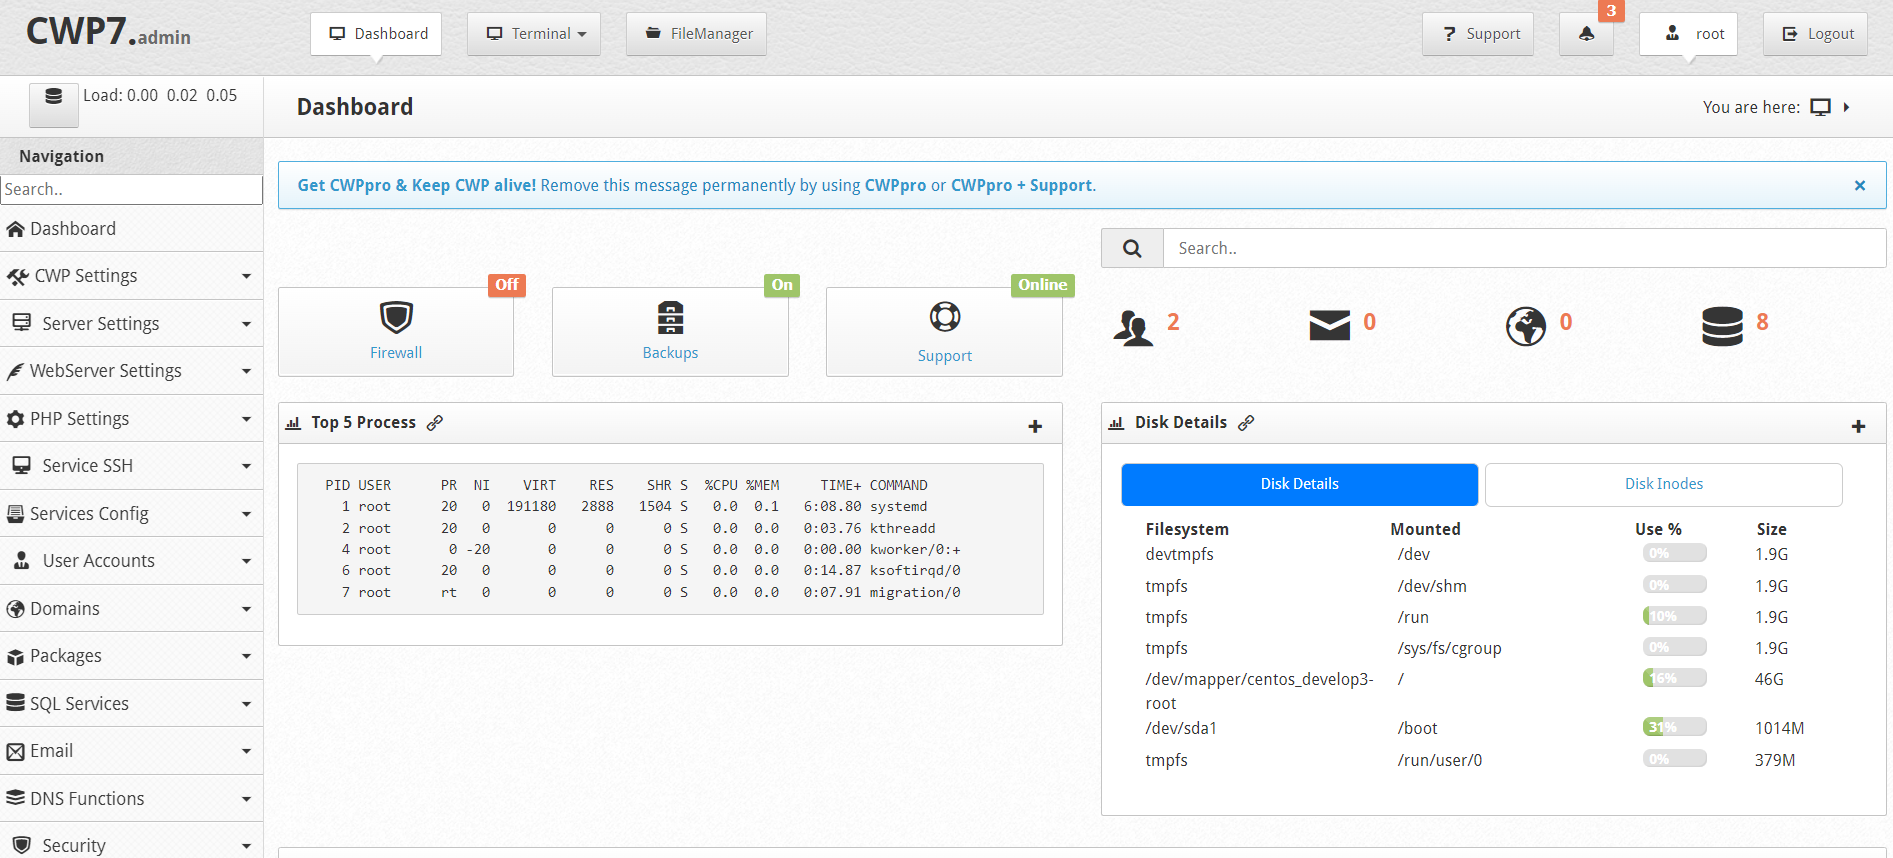
\includegraphics[height=0.3\textheight]{CWP_server.png}
    \caption[CWP van CentOs development server]{CWP van CentOs development server}
    \label{fig:centos_server}
\end{figure}
\subsection{\IfLanguageName{dutch}{Server}{Server}}
De tests worden uitgevoerd op een server die wordt gehost door Sinergio. De server draait op CentOS 7, waarbij bepaalde 
beveiligingsfunctionaliteiten tijdelijk zijn uitgeschakeld om de tests correct te kunnen uitvoeren. Zo is er op de server 
geen firewall actief en is ModSecurity ook uitgeschakeld zoals je kan zien op deze foto \ref{fig:centos_server}. Dit is gedaan om te voorkomen dat het IP-adres van de tester wordt 
geblokkeerd tijdens het simuleren van een brute force-aanval bijvoorbeeld.

ModSecurity is een open-source webapplicatie firewall (WAF) die bescherming biedt tegen verschillende soorten aanvallen door 
verdachte HTTP-verzoeken te filteren en blokkeren. Het wordt vaak gebruikt om applicaties te beschermen tegen bedreigingen 
zoals SQL-injecties, XSS-aanvallen en brute force-aanvallen. Door ModSecurity tijdelijk uit te schakelen, kunnen de testen 
worden uitgevoerd zonder dat de ingebouwde beveiligingsmaatregelen onbedoeld interfereren met de testresultaten.

Bovenop de CentOs 7 server is er een Control Web Panel (CWP) geïnstalleerd. Dit is een gratis webhosting controlepaneel dat
een grafische interface biedt voor het beheren van webhosting servers. CWP biedt een breed scala aan functies zoals
servermonitoring, bestandsbeheer en e-mailbeheer, waardoor het een handige tool is voor het beheren van webhostingomgevingen.
CentOs wordt bij Sinergio gebruikt als development server, waarbij de server wordt gebruikt voor het testen van webapplicaties 
voor ze naar productie worden overgeplaatst. De andere servers worden ondersteund door Linux 8, waarbij de server wordt 
gebruikt voor het hosten van productieomgevingen.

\subsection{\IfLanguageName{dutch}{Wordpress}{Wordpress}}
WordPress is een veelzijdig contentmanagementsysteem (CMS) dat wereldwijd wordt gebruikt door miljoenen websites, variërend van 
eenvoudige blogs tot uitgebreide e-commerceplatforms. De aantrekkingskracht van WordPress ligt in de gebruiksvriendelijke 
interface en de enorme flexibiliteit die het biedt. Gebruikers kunnen kiezen uit duizenden thema's en plugins om hun site 
naar wens aan te passen, zonder dat er programmeerkennis nodig is. Bovendien is WordPress open-source, wat betekent dat de 
gemeenschap voortdurend bijdraagt aan de verbetering en veiligheid van het platform. Dankzij de combinatie van gebruiksgemak, 
aanpasbaarheid en de brede ondersteuning door de gemeenschap blijft WordPress de voorkeur genieten van zowel beginnende als 
ervaren webontwikkelaars.

Een belangrijke aanvulling op WordPress is de Wordfence-plugin, een populaire beveiligingstool die specifiek is ontworpen 
voor WordPress-websites. Wordfence biedt uitgebreide bescherming tegen malware, brute force-aanvallen en andere online 
bedreigingen die websites kunnen treffen. Met functies zoals firewallregels, malware-scanning en inlogbeveiliging helpt 
Wordfence gebruikers om hun sites veilig en betrouwbaar te houden. Door de integratie van deze beveiligingslagen kunnen 
website-eigenaren zich richten op het creëren van content en het beheren van hun online aanwezigheid, terwijl ze gerust 
kunnen zijn over de beveiliging van hun website.

\subsection{\IfLanguageName{dutch}{Laravel}{Laravel}}
Laravel is een krachtig en veelzijdig PHP-framework dat populair is onder ontwikkelaars voor het bouwen van robuuste 
webapplicaties. Het staat bekend om zijn elegantie en eenvoud, zoals beschreven wordt in \nameref{sec:Webomgevingen} 
uit de literatuurstudie, waardoor het zowel beginners als ervaren ontwikkelaars 
aanspreekt. Laravel biedt een rijke set aan tools en bibliotheken die het ontwikkelen van complexe toepassingen eenvoudiger 
maken, zoals ingebouwde authenticatie, routing en een intuïtief templating-systeem. Het framework volgt de MVC-architectuur 
(Model-View-Controller), wat zorgt voor een gestructureerde en onderhoudbare codebase. Bovendien stimuleert Laravel het 
gebruik van best practices in webontwikkeling, zoals beveiligde codering en testen, waardoor het een betrouwbare keuze is 
voor het bouwen van veilige en schaalbare applicaties. Dankzij de uitgebreide documentatie en een actieve gemeenschap, kunnen 
ontwikkelaars snel aan de slag en blijven ze ondersteund tijdens het ontwikkelproces.

\begin{figure}
    \centering
    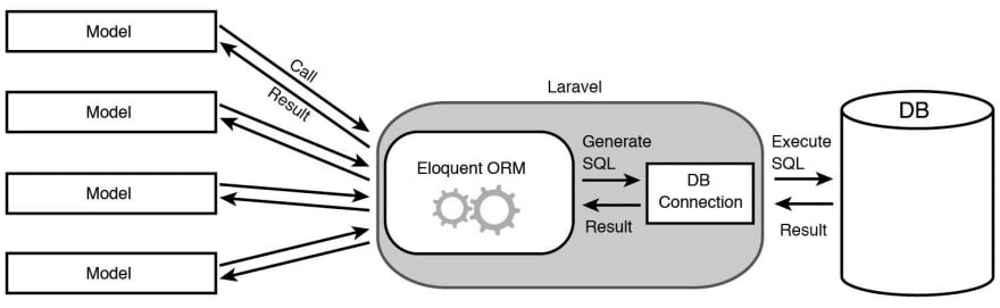
\includegraphics[height=0.2\textheight]{laravel_schema.png}
    \caption[Laravel schema]{Laravel schema}
    \label{fig:laravel_schema}
\end{figure}

Ook het ORM (Object Relational Mapping) systeem van Laravel is een belangrijke troef. Dit systeem maakt het mogelijk om 
om het systeem te beschermen van SQL-injectie via de Eloquent ORM. Dit gebeurt door middel van PDO (PHP Database Objects) binding, waarbij de
gebruiker geen directe SQL queries kan uitvoeren, doordat Eloquent de SQL commando's eerst opslaagt en de onveilige opslaagt 
als tekst. Dit is een belangrijke beveiligingsmaatregel die Laravel biedt om de veiligheid van de applicatie te garanderen.
Het schema van Laravel is te zien op deze foto \ref{fig:laravel_schema}.


\section{\IfLanguageName{dutch}{Proof of Concept: Gebruiksvriendelijkheid en Effectiviteit van Pentesting Tools voor Webapplicaties}{Proof of Concept: Usability and Effectiveness of Pentesting Tools for Web Applications}}

In de proof of concept testen we de drie verschillende webomgevingen met de vernoemde pentesting tools om hun bruikbaarheid en effectiviteit te evalueren. 
Deze benadering is gericht op het vergelijken van de uitkomsten van pentests in elke omgeving, waardoor kan vastgesteld worden hoe de 
beveiligingsuitdagingen en kwetsbaarheden verschillen.

\subsubsection{\IfLanguageName{dutch}{Omgevingsdiversiteit}{Environmental diversity}}
De aanpak in deze proof of concept is gebaseerd op een realistische benadering, waarbij de drie pentesting tools worden gebruikt die zijn afgestemd 
op de unieke kenmerken van elke omgeving. Het team van Sinergio begrijpt dat geen twee webomgevingen dezelfde zijn en daarom is het belangrijk om een breed scala 
aan tools in te zetten om alle mogelijke kwetsbaarheden en beveiligingsrisico's aan het licht te brengen.

Door deze diversiteit aan tools kan het team niet alleen de specifieke omgeving testen met de best passende tool, maar ook de algehele robuustheid en 
weerbaarheid van de systemen maximaliseren. Elke tool heeft zijn eigen sterke punten en specialiteiten, waardoor een uitgebreide evaluatie mogelijk 
is die verder gaat dan alleen de oppervlakte.

Door te variëren in de gebruikte tools, kan het team verschillende aanvalsscenario's simuleren en de reactie van de systemen daarop beoordelen. Dit 
stelt hen in staat om een diepgaand inzicht te krijgen in de beveiligingsstatus van elke omgeving en biedt waardevolle informatie voor het verbeteren 
van de algehele beveiliging.

\subsubsection{\IfLanguageName{dutch}{Focus van pentesttools}{Focus of the pentesttools}}
De evaluatie van de wordpress beveiligingsplugin wordt geëvalueerd met Burp Suite om op die manier de efficiëntie ervan te testen. De focus ligt op het evalueren van de weerstand 
tegen veelvoorkomende webaanvallen, zoals brute force-aanvallen en SQL-injectie. Ze analyseren hoe de plugin potentiële dreigingen behandelt met 
behulp van Burp Suite en identificeren eventuele tekortkomingen in de bescherming

OWASP ZAP helpt bij het blootleggen van kwetsbaarheden die een website zonder beveiligingsmaatregelen zou kunnen hebben. De nadruk ligt op het 
ontdekken van eenvoudig te exploiteren kwetsbaarheden en het trainen van aan nieuwe gebruikers om deze kwetsbaarheden te begrijpen en 
te leren hoe ze tegen te gaan.

Met Metasploit wordt gefocust op geavanceerdere beveiligingsaspecten, zoals routebescherming en authenticatiemechanismen.
In Laravel is het bijvoorbeeld mogelijk om het aantal mislukte inlogpogingen in te stellen voordat een gebruiker tijdelijk wordt geblokkeerd. Dit wordt vaak gedaan 
als een beveiligingsmaatregel om brute force-aanvallen te voorkomen. Je kunt het aantal inlogpogingen aanpassen door een eigenschap genaamd 
'maxAttempts' in te stellen in de configuratie van het authenticatiesysteem van Laravel. Deze tests zullen 
bijdragen aan het inzicht in de robuustheid van de beveiliging en helpen bij het identificeren van potentieel over het hoofd geziene kwetsbaarheden.

\section{\IfLanguageName{dutch}{Hoe pentesten}{How to pentest}}
Dit hoofdstuk beschrijft de methodologie die wordt gehanteerd voor het uitvoeren van penetratietesten op webapplicaties met behulp van Metasploit, 
Burp Suite Community Edition en OWASP ZAP. De focus ligt hierbij op twee specifieke aanvalstechnieken: brute force-aanvallen en SQL-injecties. 
Het gebruik van deze tools en technieken heeft tot doel inzicht te verkrijgen in de kwetsbaarheden van webapplicaties en de effectiviteit van 
verschillende beveiligingsmaatregelen.

\subsection{\IfLanguageName{dutch}{Voorbereiding van de testomgeving}{Voorbereiding van de testomgeving}}
Voor de uitvoering van de penetratietesten werd een gecontroleerde omgeving opgezet door Sinergio. Deze omgeving omvat een webserver waarop kwetsbare 
applicaties draaien, specifiek ontworpen om te dienen als testdoelen voor beveiligingsanalyses. Hiervoor is de server security via de firewall ook uitgezet zodat 
het IP nooit geblacklist zou worden wanneer een brute-force aanval wordt gesimuleerd. De gebruikte testapplicaties zijn gebaseerd 
op WordPress en Laravel, aangezien deze veelvoorkomende platforms representatief zijn voor echte wereldscenario's.

\subsection{\IfLanguageName{dutch}{Werkwijze metasploit}{Working method metasploit}}
Metasploit kan geïnstalleerd worden op een Windows-systeem. De installatie omvat de nieuwste versie van Metasploit Framework, samen met de 
benodigde updates en dependencies.

\subsubsection{\IfLanguageName{dutch}{Brute-force aanval}{Brute-force attack}}
Om een brute force-aanval uit te voeren met Metasploit op een webapplicatie, wordt gebruikgemaakt van de auxiliary\slash scanner\slash http\slash brute\_dirs
module. Deze module probeert verschillende URL-paden op de webserver te vinden door middel van brute force.
Het te volgen parcours gaat als volgt:
\begin{enumerate}
    \item Start Metasploit en laad de brute\_dirs module
    \begin{enumerate}
        \item msfconsole
        \item use auxiliary\slash scanner\slash http\slash brute\_dirs
    \end{enumerate}
    \item Configureer de module met de doelhost en eventuele andere parameters
    \begin{enumerate}
        \item set RHOSTS (doel-IP)
        \item set THREADS 10
        \item set PATHS (pad-naar-bestand-met-directories)
        \item set PORTS 443\slash 80 
    \end{enumerate}
    \item run
\end{enumerate}
\subsection{\IfLanguageName{dutch}{Werkwijze burp-suite community edition}{Working method  burp-suite community edition}}
Burp Suite Community Edition kan eveneens geïnstalleerd worden op een Windows-systeem. De installatie omvat de configuratie 
van de ingebouwde proxy om het HTTP-verkeer tussen de browser en de webapplicatie te onderscheppen en te analyseren.

\subsubsection{\IfLanguageName{dutch}{Brute-force aanval}{Brute-force attack}}
Met Burp Suite kan een brute force-aanval worden uitgevoerd via de 'Intruder' tool. Hierbij wordt via verschillende wachtwoordcombinaties 
getracht om toegang te verkrijgen tot de webapplicatie. Het proces verloopt als volgt:
\begin{enumerate}
    \item Start Burp Suite en configureer de proxy-instellingen in de browser.
    \item Ga naar de login-pagina van de doelwebapplicatie en onderschep het inlogverzoek met Burp Suite.
    \item Stuur het onderschepte verzoek naar de 'Intruder': Right-click > Send to intruder
    \item Configureer de 'Intruder' met de gewenste payloads (gebruikersnamen en wachtwoorden).
    \item Start de aanval door op 'Start attack' te klikken.
\end{enumerate}

\subsubsection{\IfLanguageName{dutch}{Sql-injection}{Sql-injection}}
Om een SQL-injectieaanval te simuleren wordt gebruikgemaakt van de 'Repeater' tool in Burp Suite. Op de onderstaande manier gemanipuleerde SQL-query's naar de 
server gestuurd.
\begin{enumerate}
    \item Intercept een HTTP-verzoek dat SQL-parameters bevat.
    \item Stuur het onderschepte verzoek naar de 'Repeater': Right-click > Send to repeater
    \item Manipuleer de SQL-parameter in de 'Repeater' en stuur het aangepaste verzoek naar de server.
    \item Analyseer de reactie om te bepalen of de SQL-injectie succesvol was.
\end{enumerate}

\subsection{\IfLanguageName{dutch}{Werkwijze OWASP ZAP}{Working method OWASP ZAP}}
OWASP ZAP kan eveneens geïnstalleerd worden op een Windows-systeem. De installatie omvat het configureren van de ingebouwde 
proxy om het HTTP-verkeer te onderscheppen en te analyseren.
\subsubsection{\IfLanguageName{dutch}{Brute-force aanval}{Brute-force attack}}
OWASP ZAP bevat een ingebouwde tool voor het uitvoeren van brute force-aanvallen op webapplicaties.
De configuratie verloop als volgt:
\begin{enumerate}
    \item Start OWASP ZAP en configureer de proxy-instellingen in de browser.
    \item Ga naar de login-pagina van de doelwebapplicatie en onderschep het inlogverzoek met OWASP ZAP.
    \item Klik met de rechtermuisknop op het onderschepte verzoek en selecteer 'Attack' > 'Forced Browse Site'
    \item Configureer de brute force-instellingen en start de aanval.
\end{enumerate}

\subsubsection{\IfLanguageName{dutch}{Sql-injectie}{Sql-injection}}
Voor een SQL-injectieaanval wordt gebruikgemaakt van de 'Active Scan' feature van OWASP ZAP.
De te nemen stappen zijn daar:
\begin{enumerate}
    \item Intercepteer een HTTP-verzoek dat SQL-parameters bevat.
    \item Voeg het verzoek toe aan de scan queue door met de rechtermuisknop te klikken en 'Attack' > 'Active Scan' te selecteren
    \item Start de actieve scan en analyseer de resultaten om te bepalen of er SQL-injectie kwetsbaarheden zijn.
\end{enumerate}